\documentclass{ctexart}
\usepackage{graphicx} % Required for inserting images

\title{这是一个标题}


\begin{document}

\maketitle
\begin{abstract}
    下面是这篇论文的摘要
\end{abstract}
\section{问题背景与问题需求}

\subsection{问题背景}

中药材在采收及初加工过程中通常含有较高水分，若不能及时、合理地降低其含水量，
可能对后续储藏、运输及品质稳定性产生不利影响。因此，干燥是中药材产地初加工过程中的
重要环节之一。当前中药材干燥方式主要包括自然干燥、热风干燥、真空干燥、微波干燥以及
多种联合干燥技术。其中，热风干燥由于设备结构相对简单、技术成熟且适用范围较广，
在实际生产中具有重要应用价值\cite{wang2024drying,nurhaslina2022review}。
已有研究表明，合理选择干燥工艺及相关装备，对于提高中药材干燥效率和保障成品品质
具有重要意义\cite{wang2024drying}。

在热风干燥过程中，药材与周围热空气之间持续进行热量和水分交换。一方面，
热量通过对流换热由环境传递至药材表面，并进一步通过热传导向药材内部传递；
另一方面，药材内部水分在浓度梯度作用下向表面迁移，并通过表面对流传质进入周围空气。
因此，药材烘干本质上属于具有明显时间和空间变化特征的非稳态热--质传递过程。
现有干燥理论通常以能量守恒、Fourier 热传导定律和 Fick 扩散定律等作为建立
热质传递模型的重要理论基础\cite{yan2026heat,srikiatden2007moisture}。

药材内部水分迁移过程受到干燥温度、环境湿度、材料结构、水分浓度以及有效扩散系数
等多种因素共同影响。随着干燥过程持续进行，药材内部水分不断减少，其热物性参数及
几何尺寸也可能发生变化，使热量和水分传递表现出较强的非线性特征
\cite{yan2026heat,srikiatden2007moisture}。
因此，仅依靠传统试验方法寻找适宜的烘干条件通常需要大量实验和较长周期，而利用
数学模型描述药材内部温度场和水分浓度场的动态变化，可以为烘干时间预测、
工艺参数分析以及烘干过程优化提供理论依据。

基于上述背景，本文针对题目所给近似圆柱形中药材，综合考虑热传导、水分扩散、
表面对流换热与传质以及干燥过程中尺寸变化等因素，建立药材烘干过程温度场和
水分浓度场的数学模型。通过数值计算研究温度与水分浓度随时间和空间位置的变化规律，
并进一步确定满足规定水分浓度要求时所需的烘干时间。


\begin{figure}[htbp]
    \centering
    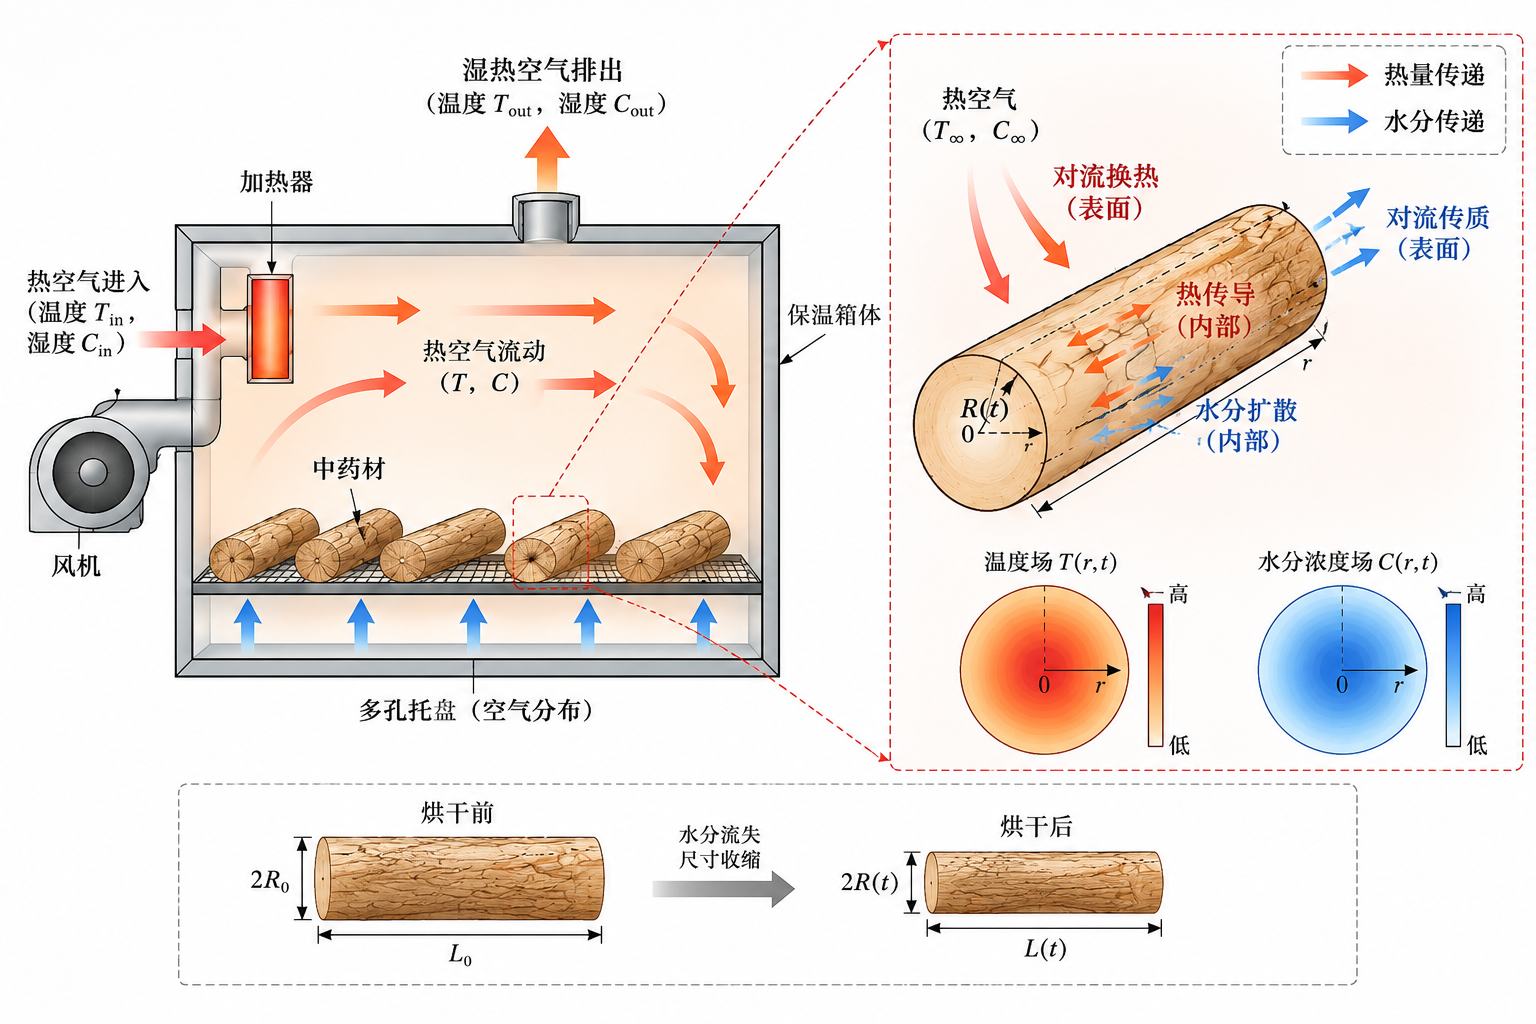
\includegraphics[width=0.96\textwidth]
    {背景.png}
    \caption{热风烘干过程中中药材的热质传递机理示意}
    \label{fig:drying-mechanism}
\end{figure}


\subsection{问题需求}

研究对象为一根近似圆柱形的中药材，其初始长度为 $25\,\mathrm{cm}$，
半径为 $2\,\mathrm{cm}$，初始温度为 $28\,^{\circ}\mathrm{C}$，
初始干基水分浓度为 $2.55\,\mathrm{kg/kg}$。
在给定烘房温度、水分浓度以及相关热物性和传质参数的条件下，
需要研究药材内部温度和水分浓度随时间及空间位置的变化规律。
结合题目要求，需要依次解决以下四个问题。

\textbf{问题一：预热平衡阶段的温度和水分浓度变化规律。}

根据烘房温度和水分浓度随时间的变化数据，建立药材预热阶段的非稳态传热与
传质模型。在给定初始条件和边界条件下，求解药材不同径向位置处的温度
$T(r,t)$ 和水分浓度 $C(r,t)$，获得 $1800\,\mathrm{s}$ 内药材内部
温度场和水分浓度场的时空变化规律。

\textbf{问题二：完整烘干过程的温度和水分浓度变化规律。}

在问题一模型的基础上，将研究范围扩展至预热平衡和恒温干燥全过程。
考虑密度 $\rho$、比热容 $c_p$、热传导系数 $k$ 以及水分扩散系数 $D$
随药材温度和水分浓度发生变化，建立具有变物性参数的热--质传递模型，
研究完整烘干过程中温度场和水分浓度场的动态演化规律。

\textbf{问题三：确定满足烘干要求的最短烘干时间。}

以药材内部各位置的水分浓度均低于
$0.15\,\mathrm{kg/kg}$ 作为烘干完成条件。
利用问题二建立的数学模型计算不同时间和不同径向位置处的水分浓度，
通过判断药材内部最大水分浓度是否满足给定阈值，确定满足烘干要求所需的
最短烘干时间。

\textbf{问题四：考虑尺寸收缩后的烘干过程。}

在实际烘干过程中，随着水分不断流失，药材会发生尺寸收缩。
因此，在前三问模型基础上进一步引入药材半径随时间的变化关系 $R(t)$，
建立具有移动边界特征的水分迁移模型，重新计算药材内部水分浓度分布和最终
烘干时间，并分析尺寸变化对药材烘干过程的影响。

\section{模型假设}

\section{符号说明}

\section{模型建立与问题求解}

\subsection{问题1：预热平衡阶段药材温度、水分浓度变化模型}

\subsubsection{控制方程与定解条件}

预热平衡阶段（前 30 min）药材与烘房热空气之间进行非稳态热--质交换：热量经表面对流
换热进入药材并沿径向向内传导，水分则在浓度梯度作用下由内向外扩散、经表面对流传质
进入空气\cite{yan2026heat,srikiatden2007moisture}。药材为长 $25\,\mathrm{cm}$、
半径 $2\,\mathrm{cm}$ 的细长圆柱（长径比 $6.25$），侧面受热风均匀吹拂，
且题目要求的输出自变量为“到药材中心的距离”，故将问题简化为\textbf{轴对称一维径向
热传导--水分扩散模型}。按问题 1 要求，物性取附录 2 给定常数
（$\rho$、$c_p$、$k$ 与 $C$ 无关，$D$ 仅依赖水分浓度、不含温度 Arrhenius 项），
因此温度场与水分场仅通过边界条件耦合，两方程可分别求解。控制方程与定解条件为
\begin{equation}
  \rho c_p\frac{\partial T}{\partial t}
  =\frac{1}{r}\frac{\partial}{\partial r}\Big(k r\frac{\partial T}{\partial r}\Big),
  \qquad 0<r<R,\ t>0,
  \label{eq:heat}
\end{equation}
\begin{equation}
  \frac{\partial C}{\partial t}
  =\frac{1}{r}\frac{\partial}{\partial r}\Big(D(C)\,r\frac{\partial C}{\partial r}\Big),
  \qquad 0<r<R,\ t>0,
  \label{eq:moist}
\end{equation}
其中水分扩散系数按附录 2 取经验公式（注意指数为 $-0.89/C$ 而非 $-0.89C$）
\begin{equation}
  D(C)=7\times10^{-9}\exp\!\Big(-\frac{0.89}{C}\Big).
  \label{eq:D}
\end{equation}
初始条件为全场均匀：
\begin{equation}
  T(r,0)=28\,^{\circ}\mathrm{C},\qquad C(r,0)=2.55\ \mathrm{kg/kg}.
  \label{eq:ic}
\end{equation}
边界条件为：圆心处轴对称零梯度，表面为第三类对流换热与对流传质：
\begin{equation}
  \frac{\partial T}{\partial r}(0,t)=\frac{\partial C}{\partial r}(0,t)=0,
  \label{eq:bc0}
\end{equation}
\begin{equation}
  -k\frac{\partial T}{\partial r}(R,t)=h\big[T(R,t)-T_a(t)\big],
  \qquad
  -D(C_s)\frac{\partial C}{\partial r}(R,t)=h_m\big[C_s(t)-C_a(t)\big],
  \label{eq:bcR}
\end{equation}
式中 $T_a(t)$、$C_a(t)$ 为附件 1 给出的烘房温度与水分浓度时变序列，$C_s(t)=C(R,t)$
为表面水分浓度。\eqref{eq:moist} 右端的 $D(C)$ 必须保留在散度之内，展开后含
$D'(C)(\partial C/\partial r)^2$ 非线性项，简单写作 $D\Delta C$ 会丢失该
“越干扩散越慢”的自锁效应。

\subsubsection{物性参数与烘房条件}

按附录 2，第一问全部物性参数如表~\ref{tab:params} 所示，无任何待定参数，其量级与文献报道的中药材热风干燥物性一致\cite{wang2024drying}；
烘房环境由附件 1 给出（$0\sim14400\,\mathrm{s}$ 共 241 条、间隔 $60\,\mathrm{s}$），
本问只使用 $0\sim1800\,\mathrm{s}$ 段，相邻观测点间做分段线性插值，不平滑、不外推。
表~\ref{tab:air} 列出表 1/表 2 所要求 7 个时刻处的烘房条件（线性插值）。

\begin{table}[htbp]
  \centering
  \caption{问题 1 物性参数（附录 2）}
  \label{tab:params}
  \begin{tabular}{lll}
    \hline
    参数 & 数值 & 单位 \\
    \hline
    密度 $\rho$ & 820 & $\mathrm{kg/m^3}$ \\
    比热容 $c_p$ & 2600 & $\mathrm{J/(kg\cdot K)}$ \\
    导热系数 $k$ & 0.36 & $\mathrm{W/(m\cdot K)}$ \\
    对流换热系数 $h$ & 25 & $\mathrm{W/(m^2\cdot K)}$ \\
    对流传质系数 $h_m$ & $8\times10^{-7}$ & $\mathrm{m/s}$ \\
    水分扩散系数 $D$ & $7\times10^{-9}\exp(-0.89/C)$ & $\mathrm{m^2/s}$ \\
    半径 $R$／长度 $L$ & 0.02／0.25 & $\mathrm{m}$ \\
    初始温度／水分浓度 & 28／2.55 & $^{\circ}\mathrm{C}$／$\mathrm{kg/kg}$ \\
    \hline
  \end{tabular}
\end{table}

\begin{table}[htbp]
  \centering
  \caption{附件 1 烘房条件（表 1/表 2 要求时刻，线性插值）}
  \label{tab:air}
  \begin{tabular}{cccccccc}
    \hline
    $t/\mathrm{s}$ & 100 & 300 & 600 & 900 & 1200 & 1500 & 1800 \\
    \hline
    $T_a/^{\circ}\mathrm{C}$ & 28.9707 & 30.8340 & 33.2020 & 35.5240 & 37.8820 & 39.5950 & 41.5130 \\
    $C_a/(\mathrm{kg/kg})$ & 0.02036 & 0.02191 & 0.02428 & 0.02660 & 0.02891 & 0.03098 & 0.03307 \\
    \hline
  \end{tabular}
\end{table}

\begin{figure}[htbp]
  \centering
  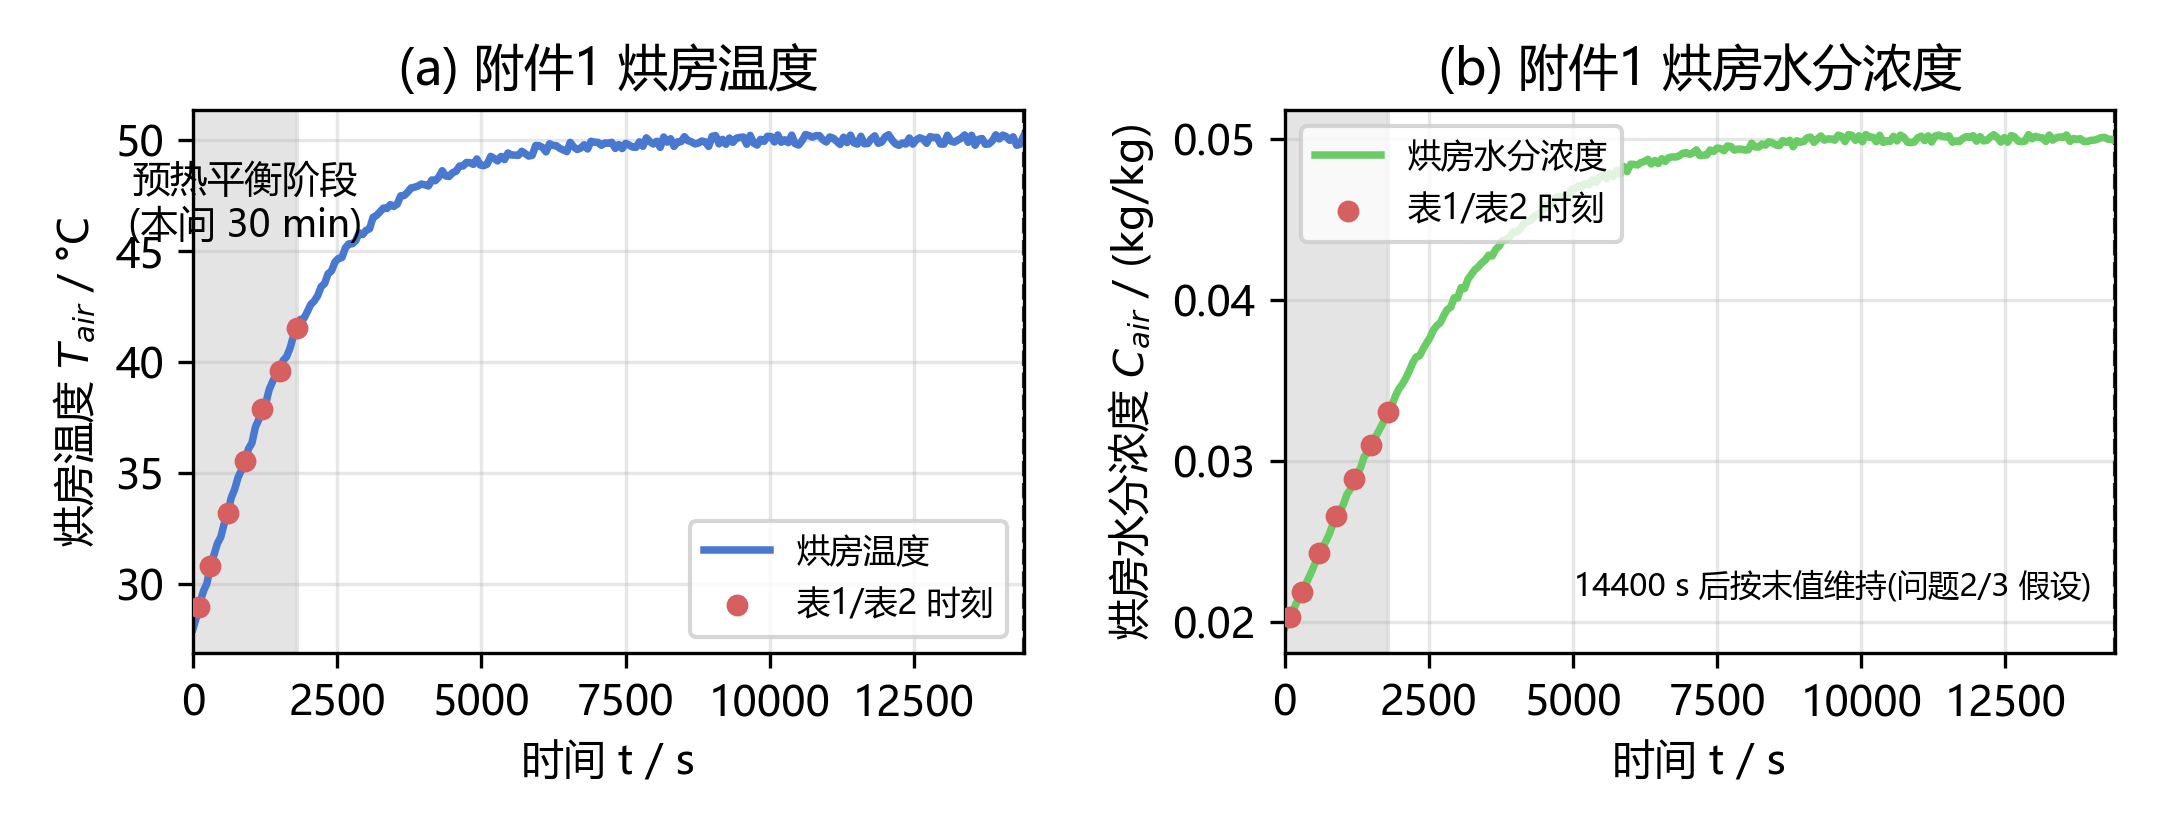
\includegraphics[width=0.85\textwidth]{fig01_chamber.png}
  \caption{附件 1 烘房条件：阴影为本问 30 min 考察窗，圆点为表 1/表 2 要求时刻}
  \label{fig:chamber}
\end{figure}

\subsubsection{特征时间与量级分析（求解前的先验判断）}

求解前先以特征时间与 Biot 数对模型做量级分析，为数值结果提供锚点。热扩散率与初始
扩散系数分别为 $\alpha=k/(\rho c_p)=1.6886\times10^{-7}\ \mathrm{m^2/s}$ 与
$D(C_0)=7\times10^{-9}e^{-0.89/2.55}=4.9377\times10^{-9}\ \mathrm{m^2/s}$，于是
\begin{equation}
  \tau_T=\frac{\rho c_pR^2}{k}=2368.9\ \mathrm{s}\approx39.5\ \mathrm{min},
  \qquad
  \tau_C=\frac{R^2}{D(C_0)}=8.10\times10^{4}\ \mathrm{s}\approx22.5\ \mathrm{h},
  \label{eq:tau}
\end{equation}
\begin{equation}
  Bi=\frac{hR}{k}=1.389,\qquad
  Bi_m=\frac{h_mR}{D(C_0)}=3.240.
  \label{eq:bi}
\end{equation}
式中特征时间与 Biot 数是干燥研究中刻画温度场/水分场演化时间尺度及表面传质控制
机制的常用量纲分析工具\cite{yan2026heat,srikiatden2007moisture}。
由此得到三条先验判断，后文数值结果将逐条印证：
\begin{enumerate}
  \item \textbf{热快湿慢}：$\tau_C/\tau_T\approx34$，30 min 约为 $0.76\,\tau_T$ 却仅占
        $\tau_C$ 的 $2.2\%$，故 30 min 内温度场显著建立，而水分只来得及在表面薄层内变化；
  \item \textbf{内部温度梯度不可忽略}：$Bi=O(1)$，不能用集总参数法，径向温差可达数摄氏度；
  \item \textbf{表面水分迅速趋近烘房湿度}：$Bi_m=3.24>1$，失水由对流边界驱动，将形成
        表面干、内部湿的“干壳湿芯”结构。
\end{enumerate}

\begin{figure}[htbp]
  \centering
  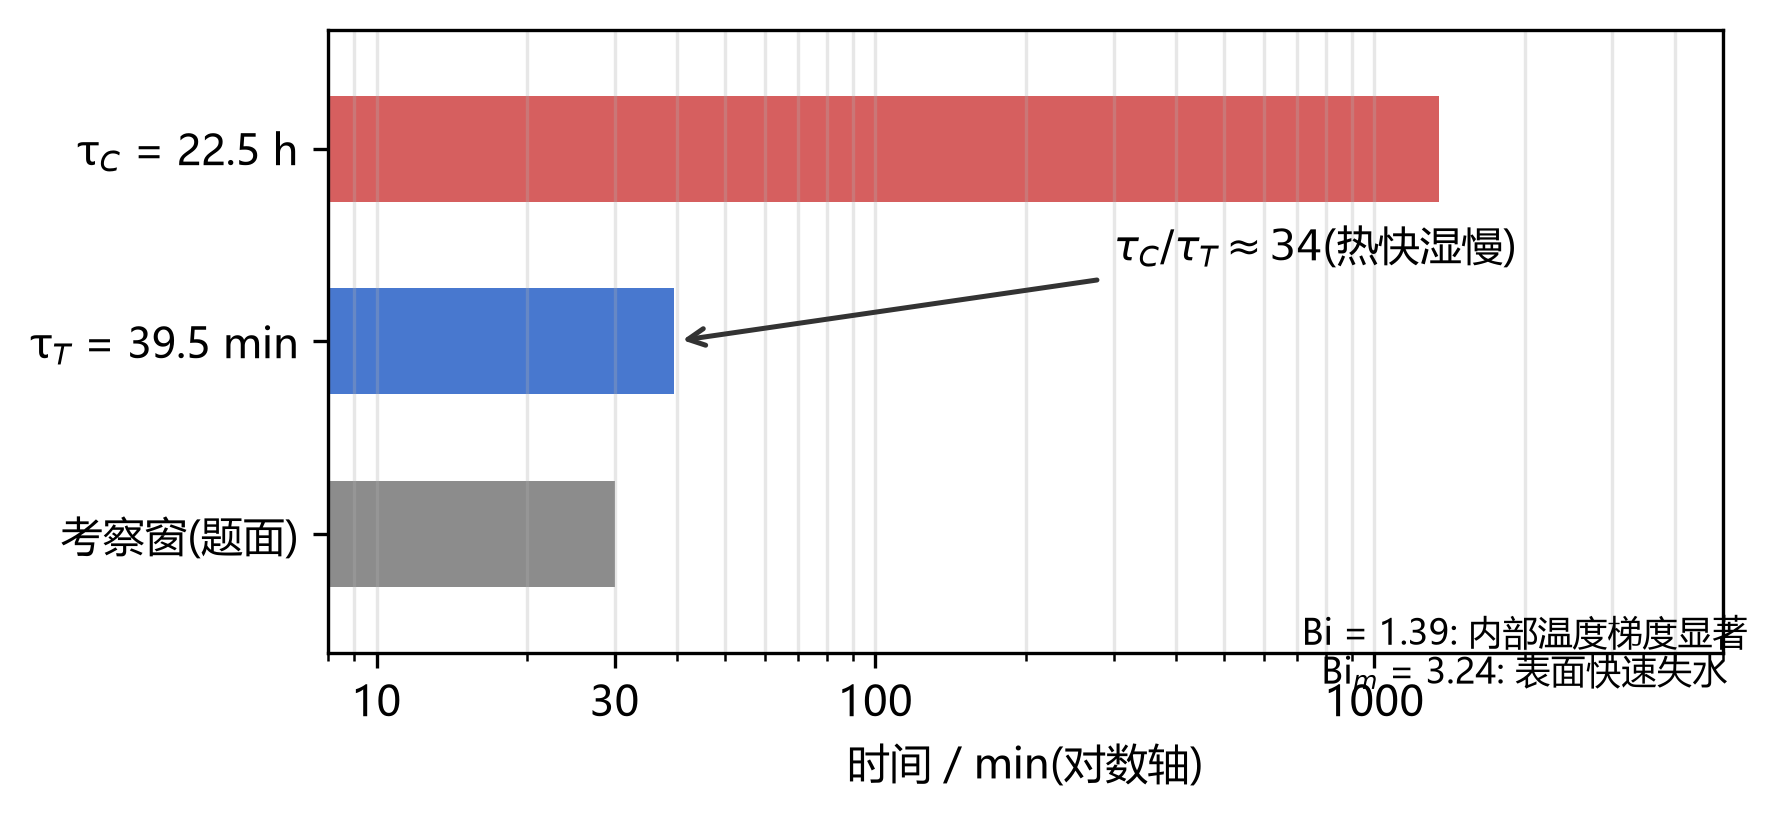
\includegraphics[width=0.75\textwidth]{fig05_timescale.png}
  \caption{特征时间量级对比（对数轴）：30 min 考察窗与 $\tau_T$ 同量级、$\tau_C$ 大 34 倍}
  \label{fig:timescale}
\end{figure}

\subsubsection{数值求解方法}

\textbf{(1) 归一化坐标与表面加密网格。}引入 $\xi=r/R$，式~\eqref{eq:heat}、\eqref{eq:moist}
化为
\begin{equation}
  \rho c_p\frac{\partial T}{\partial t}
  =\frac{1}{R^2\xi}\frac{\partial}{\partial \xi}\Big(\xi k\frac{\partial T}{\partial\xi}\Big),
  \qquad
  \frac{\partial C}{\partial t}
  =\frac{1}{R^2\xi}\frac{\partial}{\partial \xi}\Big(\xi D(C)\frac{\partial C}{\partial\xi}\Big).
  \label{eq:norm}
\end{equation}
采用单元中心有限体积法离散。水分场的数值难点在于初始时刻 $C_0\neq C_a(0)$ 引起的
表面边界层：其厚度按自相似估计为 $\delta_\theta(t)=\sqrt{\pi D t}$，
$t=10\,\mathrm{s}$ 时仅 $3.9\times10^{-4}\,\mathrm{m}$，$t=1800\,\mathrm{s}$ 时为
$1.7\times10^{-3}\,\mathrm{m}$。为使网格始终分辨该薄层，取表面加密网格
\begin{equation}
  \xi_{j+1/2}=1-\Big(1-\frac{j}{N}\Big)^2,\qquad j=0,1,\dots,N,\quad N=800,
  \label{eq:mesh}
\end{equation}
其最外单元中心距真实表面 $1.25\times10^{-5}\,\mathrm{m}$，比最薄的边界层还细约 30 倍；
计算仍使用精确环形体积权重 $V_i=(\xi_{i+1/2}^2-\xi_{i-1/2}^2)/2$。

\textbf{(2) 界面通量与边界闭性。}界面 $f$ 的通量取
$\Phi_f=G_f(u_{f-1}-u_f)$，$G_f=\xi_f\bar D_f/\Delta\xi$。对非线性 $D(C)$，界面等效
系数的精确形式为对数平均 $\bar D_{\log}=(D_1-D_2)/\ln(D_1/D_2)$；对本题
$D=Ae^{-a/C}$，对数平均与调和平均 $\bar D_{\mathrm{harm}}=2D_1D_2/(D_1+D_2)$ 按
$\varepsilon=\ln(D_2/D_1)$ 展开到 $\varepsilon^2$ 完全相同（恰为离散格式自身的截断阶），
故内部界面采用计算量更小的调和平均；积分通量（Kirchhoff 变换）路径独立，作为校核通道
保留\cite{srikiatden2007moisture}。表面采用串联热阻精确闭性：单元中心到表面的半单元导热与对流传热串联，
\begin{equation}
  G_N=\frac{1}{\dfrac{\ln(1/\xi_{c,N})}{k}+\dfrac{1}{hR}},
  \label{eq:GN}
\end{equation}
水分边界同理（以 $D_N$ 与 $h_mR$ 串联），表面值由通量一致性反解
$T_s=T_a+\Phi_N/(hR)$、$C_s=C_a+\Phi_{C,N}/(h_mR)$，比线性外推精度高约一个量级。

\textbf{(3) 时间推进与误差预算。}采用全隐式后向 Euler 与阻尼 Newton 迭代
（三对角线性化、解析 Jacobian），每个候选大步分别以整步与两个半步计算并比较全场
最大差 $e$ 实现步长加倍误差控制：接受时保留两次半步解，下一步长按误差比调整。
温度与水分各取时间误差预算 $\varepsilon=2.5\times10^{-5}$（分别以 $^{\circ}\mathrm{C}$、
$\mathrm{kg/kg}$ 计），最大步长 $1\,\mathrm{s}$，并在每个整秒输出点与输入分段节点前
截断步长。温度、水分方程在问题 1 中解耦，分别推进。

\textbf{(4) 输出采样。}内部目标点由单元中心值局部二次插值获得；表面点按 (2) 反解；
$t=0$ 行作为初始状态单独保留，Excel 按附件 3 模板自 $t=1\,\mathrm{s}$ 起输出；全部
数值四舍五入至 4 位小数后写出 $1800\times21$ 的完整时空分布至 result1.xlsx。

\subsubsection{结果与分析}

表~\ref{tab:T1} 与表~\ref{tab:C1} 给出题目要求格式的 7 个时刻、5 个径向位置处的温度与
水分浓度。

\begin{table}[htbp]
  \centering
  \caption{表 1\quad 30 分钟内药材的温度（$^{\circ}\mathrm{C}$）}
  \label{tab:T1}
  \begin{tabular}{cccccc}
    \hline
    时间/s & \multicolumn{5}{c}{到药材中心的距离/cm} \\
    & 0 & 0.5 & 1 & 1.5 & 2 \\
    \hline
    100   & 28.0001 & 28.0003 & 28.0040 & 28.0327 & 28.1801 \\
    300   & 28.0408 & 28.0635 & 28.1514 & 28.3681 & 28.8489 \\
    600   & 28.4533 & 28.5360 & 28.8039 & 29.3159 & 30.1652 \\
    900   & 29.3243 & 29.4583 & 29.8755 & 30.6161 & 31.7304 \\
    1200  & 30.5427 & 30.7098 & 31.2224 & 32.1126 & 33.4276 \\
    1500  & 31.9957 & 32.1867 & 32.7660 & 33.7463 & 35.1203 \\
    1800  & 33.5753 & 33.7720 & 34.3642 & 35.3621 & 36.7856 \\
    \hline
  \end{tabular}
\end{table}

\begin{table}[htbp]
  \centering
  \caption{表 2\quad 30 分钟内药材的水分浓度（$\mathrm{kg/kg}$）}
  \label{tab:C1}
  \begin{tabular}{cccccc}
    \hline
    时间/s & \multicolumn{5}{c}{到药材中心的距离/cm} \\
    & 0 & 0.5 & 1 & 1.5 & 2 \\
    \hline
    100   & 2.5500 & 2.5500 & 2.5500 & 2.5500 & 2.2470 \\
    300   & 2.5500 & 2.5500 & 2.5500 & 2.5492 & 2.0508 \\
    600   & 2.5500 & 2.5500 & 2.5500 & 2.5353 & 1.8770 \\
    900   & 2.5500 & 2.5500 & 2.5497 & 2.5045 & 1.7547 \\
    1200  & 2.5500 & 2.5500 & 2.5482 & 2.4646 & 1.6586 \\
    1500  & 2.5500 & 2.5499 & 2.5445 & 2.4206 & 1.5787 \\
    1800  & 2.5500 & 2.5497 & 2.5383 & 2.3755 & 1.5102 \\
    \hline
  \end{tabular}
\end{table}

\begin{figure}[htbp]
  \centering
  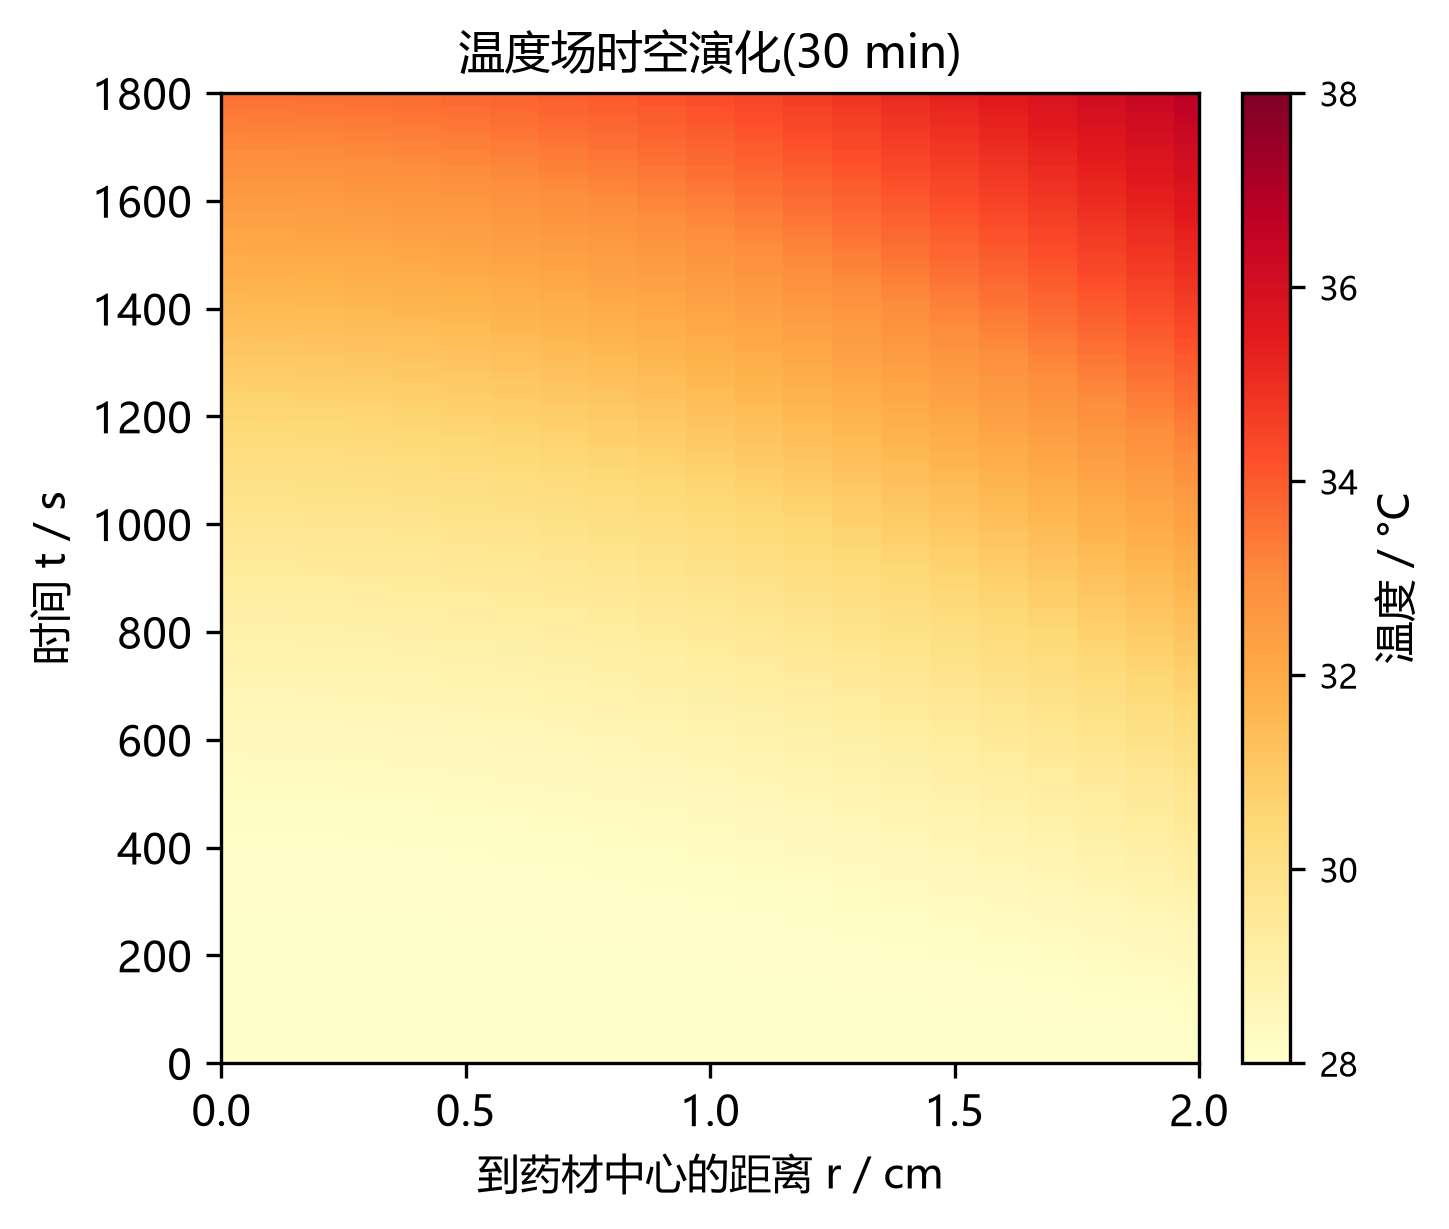
\includegraphics[width=0.72\textwidth]{fig02_temp_map.png}
  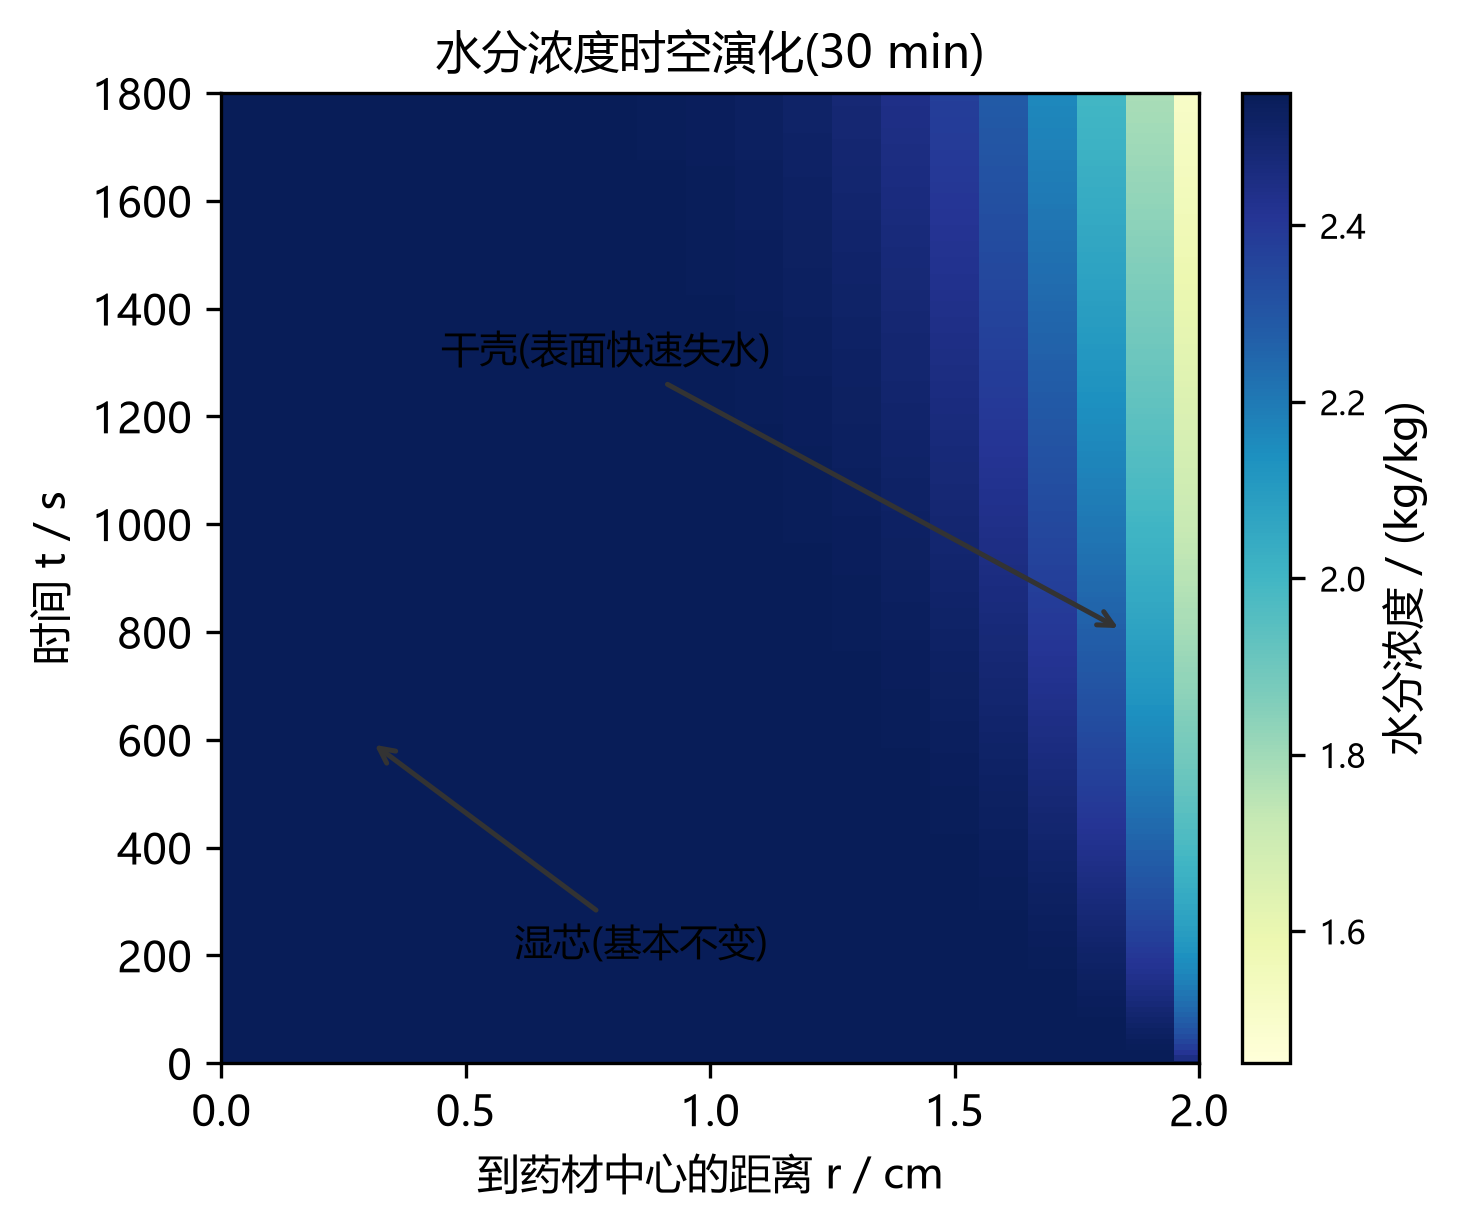
\includegraphics[width=0.72\textwidth]{fig03_moist_map.png}
  \caption{30 min 内温度场（上）与水分浓度场（下）的时空演化热力图}
  \label{fig:fields}
\end{figure}

\begin{figure}[htbp]
  \centering
  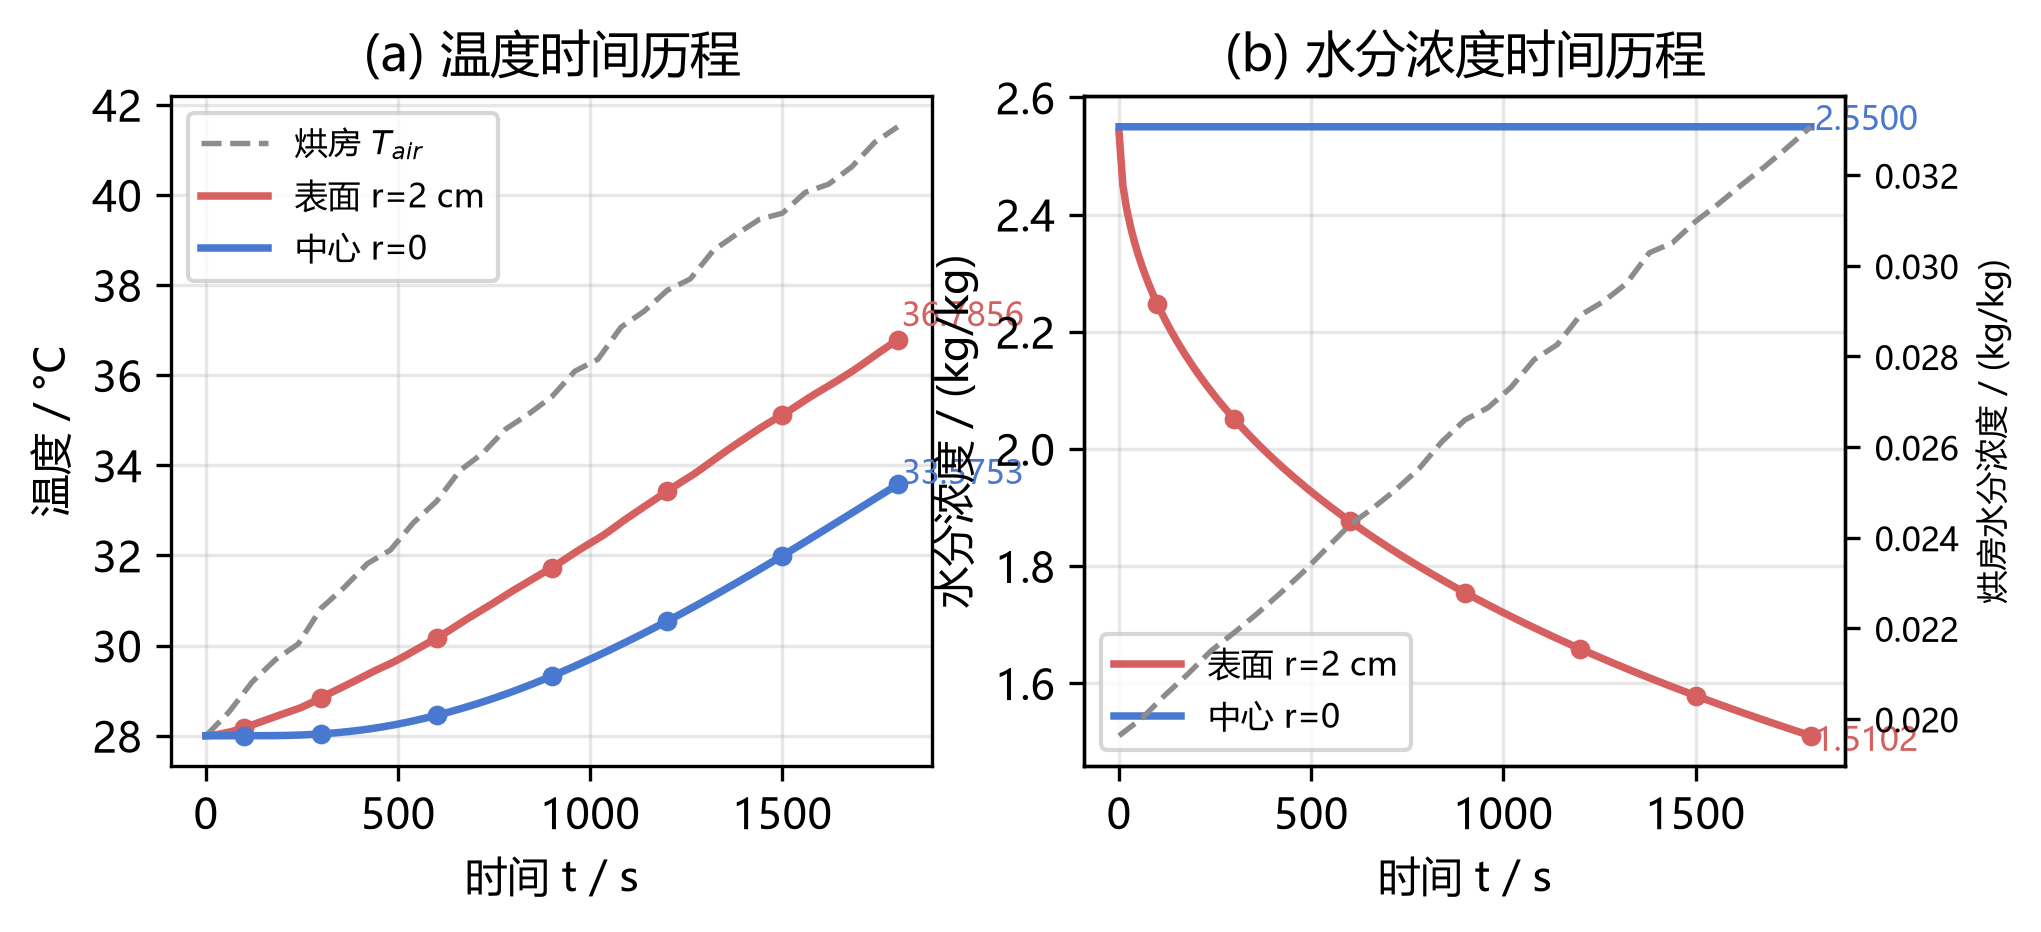
\includegraphics[width=0.8\textwidth]{fig04_timeseries.png}
  \caption{表面与中心温度、水分浓度的时间历程（圆点为表 1/表 2 要求时刻）}
  \label{fig:series}
\end{figure}

\textbf{(1) 温度场：表面先升温、中心滞后，预热平衡尚未完成。}30 min 内表面温度由
$28$ 升至 $36.7856\,^{\circ}\mathrm{C}$（升温 $8.79\,^{\circ}\mathrm{C}$），中心升至
$33.5753\,^{\circ}\mathrm{C}$（升温 $5.58\,^{\circ}\mathrm{C}$），1800 s 时径向温差达
$3.21\,^{\circ}\mathrm{C}$，与 $Bi=1.39$ 的预估一致，说明集总参数法确实不适用；
表面仍比烘房低 $41.5130-36.7856=4.73\,^{\circ}\mathrm{C}$，表明预热平衡阶段在 30 min
内尚未结束，与 $\tau_T\approx39.5\ \mathrm{min}$ 完全自洽。

\textbf{(2) 水分场：表面快速失水、内部几乎不动，呈“干壳湿芯”。}表面水分浓度由
$2.55$ 降至 $1.5102\ \mathrm{kg/kg}$（降幅 $40.8\%$），$r=1.5\ \mathrm{cm}$ 处降
$6.8\%$，$r=1.0\ \mathrm{cm}$ 处仅降 $0.46\%$，中心在 4 位小数精度下不变；水分扰动在
30 min 内仅渗入约 $0.8\ \mathrm{cm}$，显著下降（$>1\%$）局限于表面 $0.5\ \mathrm{cm}$
薄层，与 $\tau_C\approx22.5\ \mathrm{h}\gg1800\ \mathrm{s}$ 及 $Bi_m=3.24$ 的预估一致，
呈现热风干燥中典型的表层先干现象\cite{wang2024drying,nurhaslina2022review}。

\textbf{(3) 表面失水的早期快降。}表面水分在最初 100 s 内即下降 $11.9\%$，而
$1500\sim1800\,\mathrm{s}$ 仅降 $4.3\%$——初始失水速率最高，随后表面浓度趋近烘房
湿度（0.033 kg/kg）而放缓，是对流传质边界驱动的典型指数趋近行为，也印证了初始
时刻 $C_0\neq C_a(0)$ 引起快速初始边界层的判断。

\subsubsection{模型验证与精度保证}

\textbf{(1) 温度场的解析模态解逐点验证（最强证据）。}问题 1 物性全为常数，对分段线性
环境 $T_a(t)$ 存在精确模态解：令 $\lambda_mJ_1(\lambda_m)=Bi\,J_0(\lambda_m)$，
$A_m=2J_1(\lambda_m)/[\lambda_m(J_0^2(\lambda_m)+J_1^2(\lambda_m))]$，则
\begin{equation}
  T(r,t)=T_a(t)-\sum_{m=1}^{\infty}A_mJ_0\Big(\frac{\lambda_mr}{R}\Big)z_m(t),
  \qquad
  z_m'=T_a'-\frac{\lambda_m^2\alpha}{R^2}z_m,
  \label{eq:modal}
\end{equation}
每个 60 s 线性段内 $z_m$ 可逐段精确积分。用该解析解（不依赖数值求解器）与数值解在
全部 $1801\times21$ 个输出点上比对：\textbf{最大绝对差 $5.2916\times10^{-6}\,^{\circ}\mathrm{C}$}
（出现在 $t=780\ \mathrm{s}$、$r=0.4\ \mathrm{cm}$），模态截断（180 项 vs 360 项）
差异 $4.5\times10^{-8}\,^{\circ}\mathrm{C}$，1800 s 时中心/表面温度与解析解分别相差
$1.6\times10^{-7}$ 与 $2.6\times10^{-6}\,^{\circ}\mathrm{C}$。

\textbf{(2) 守恒收支与物理界。}离散储存量变化与边界交换量的闭合残差：显热收支相对残差
$2.0\times10^{-14}$、水分收支相对残差 $5.8\times10^{-13}$；全场温度 $\in[28.0000,
36.7856]$、水分浓度 $\in[1.5102,2.5500]$，无负值、无 NaN。

\textbf{(3) 网格/时间收敛与误差预算。}表面加密网格下 $N$ 逐级加倍，水分场观测空间收敛阶
$1.9998$（近似二阶），据此做 Richardson 外推；时间误差由同网格独立 BDF 实现比对估计。
误差预算逐级收紧（$2\times10^{-4}\to2.5\times10^{-5}$）后全场估计数值误差为
\textbf{温度 $5.336\times10^{-6}\,^{\circ}\mathrm{C}$、水分 $8.105\times10^{-6}\ \mathrm{kg/kg}$}，
均远小于 4 位小数舍入阈值 $5\times10^{-5}$，故表 1/表 2 与 result1.xlsx 的 4 位小数
可靠。上述误差是“给定模型、给定输入”下的数值误差估计，不是实验预测误差。

\textbf{(4) 早期表面水分的自相似解析核对。}半无限体对流边界的短时自相似解给出
$C_0-C_s(t)=(C_0-C_a)\cdot2h_m\sqrt{t/(\pi D)}$：$t=1\ \mathrm{s}$ 时解析值
$C_s=2.5175$，数值解 $2.5177$，相对差 $8\times10^{-5}$，说明初始边界层被网格与时间
步长（最小时步 $1.0\times10^{-10}\ \mathrm{s}$）真实分辨。

\begin{table}[htbp]
  \centering
  \caption{问题 1 验证汇总}
  \label{tab:verify}
  \begin{tabular}{lll}
    \hline
    验证项 & 方法 & 结果 \\
    \hline
    温度 vs 解析模态解 & 式~\eqref{eq:modal}，1801$\times$21 逐点 & 最大差 $5.29\times10^{-6}\,^{\circ}\mathrm{C}$ \\
    常环境解析基准 & 恒定边界级数解（$N=800$） & $3.4\times10^{-5}\,^{\circ}\mathrm{C}$／$1.5\times10^{-5}$ kg/kg \\
    收支闭合 & 储存量变化 vs 边界通量积分 & $2.0\times10^{-14}$／$5.8\times10^{-13}$ \\
    空间收敛 & $N=400\to800\to1600$ 外推 & 阶 1.9998 \\
    时间误差 & 同网格独立 BDF 比对 & $4.8\times10^{-9}$ kg/kg（$2.5\times10^{-5}$ 预算） \\
    早期边界层 & 自相似解 $t=1\ \mathrm{s}$ & 相对差 $8\times10^{-5}$ \\
    4 位小数保证 & 估计误差 vs 阈值 $5\times10^{-5}$ & 误差 $\le2\times10^{-5}$，全部可靠 \\
    \hline
  \end{tabular}
\end{table}

\begin{figure}[htbp]
  \centering
  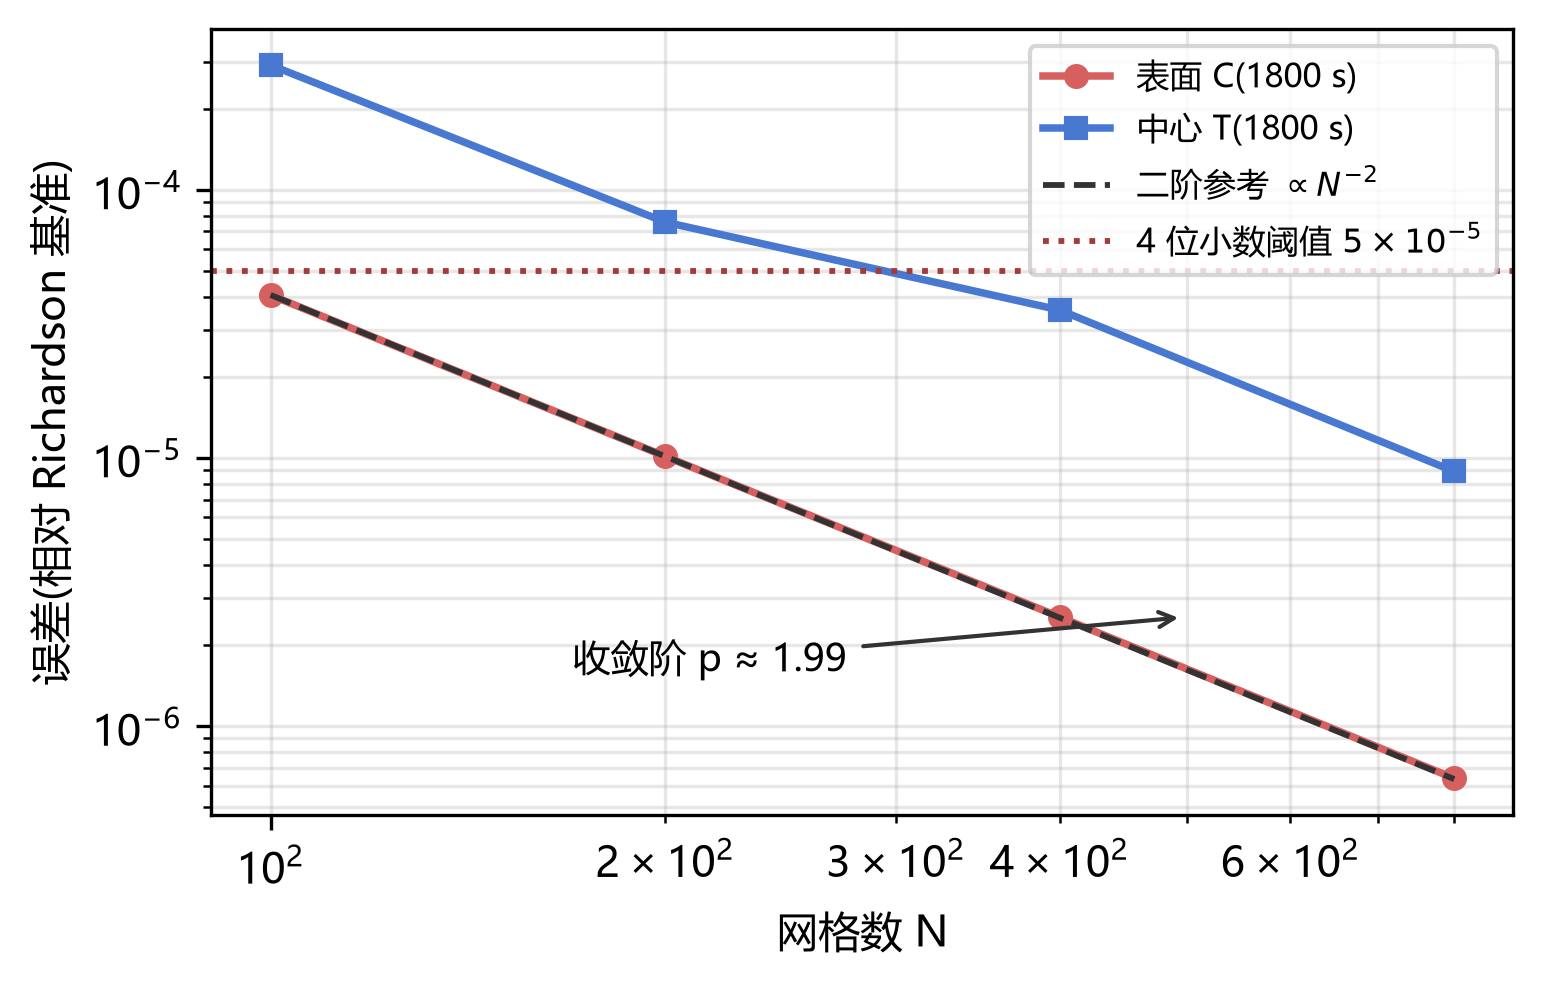
\includegraphics[width=0.72\textwidth]{fig06_convergence.png}
  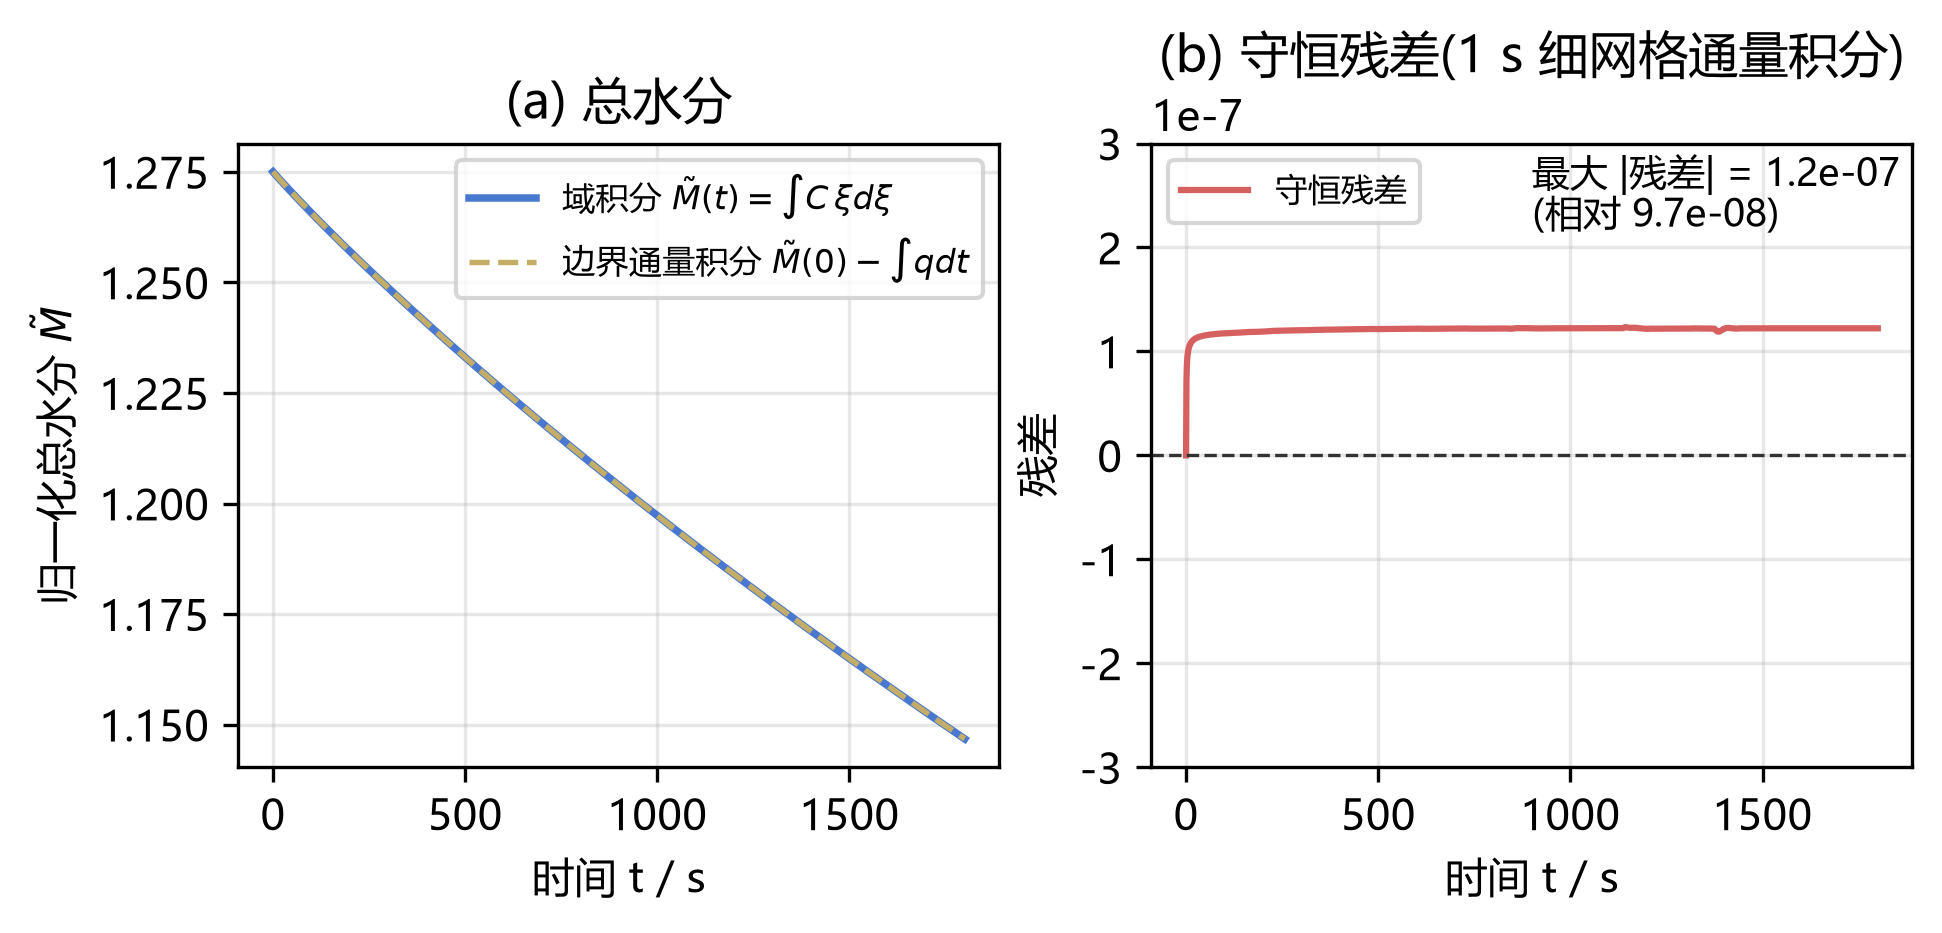
\includegraphics[width=0.72\textwidth]{fig07_conservation.png}
  \caption{网格收敛性（左）与水分质量守恒（右）}
  \label{fig:verify}
\end{figure}

\subsubsection{假设适用边界与模型误差}

本问结果建立在若干显式假设之上，其影响已尽量量化：
\begin{enumerate}
  \item \textbf{端面忽略}：端面面积约占全部换热面积的 $7.4\%$。以两端面对流换热的
        有限长圆柱解作上界情景，中截面温度与一维径向模型之差小于
        $6.3\times10^{-8}\,^{\circ}\mathrm{C}$，端部影响可忽略；
  \item \textbf{表面平衡关系 $C_e=C_a$}：题目未给吸附等温线，该等式是使用 $h_m$ 的
        有效边界闭合。敏感性计算表明 $C_e$ 抬高 $0.10\ \mathrm{kg/kg}$ 仅使表面水分
        浓度升高约 $0.85\%$——由于 $C_a\ll C_s$，问题 1 在 30 min 内对该基准歧义不敏感
        （该歧义在第三、四问长时间干燥中才会被放大）；
  \item \textbf{显热模型与蒸发潜热}：按末端表面通量估算潜热汇约 $3.65\ \mathrm{W/m^2}$，
        为显热流的 $3.1\%$，引起表面温度约 $-0.11\ \mathrm{K}$ 的变化，不改变本问
        4 位小数结论，但其对长时间干燥的影响在问题 2/3 中讨论；
  \item \textbf{半径不变}：附件 2 显示 30 min 内半径收缩 $6.35\%$，问题 1 按题面规定取
        $R=2\ \mathrm{cm}$ 常数，收缩效应由问题 4 的移动边界模型处理；
  \item \textbf{辅助统计量口径}：按模型内部 800 单元体积权平均，1800 s 时截面平均含水率为
        $2.2936\ \mathrm{kg/kg}$，对应失水约 $18.6\ \mathrm{g}$；若对交付表 21 个径向
        采样点做梯形积分则得 $2.4031$（失水 $10.7\ \mathrm{g}$）。差异源于失水集中于
        表面约 $1.7\ \mathrm{mm}$ 薄层、$0.1\ \mathrm{cm}$ 的采样间距无法分辨该层，
        本文以守恒口径（18.6 g）为准，点值表不受影响。
\end{enumerate}

综上，预热平衡阶段的药材呈“热场基本建立、水分刚启动”的过渡状态：表面温度
$28\to36.7856\,^{\circ}\mathrm{C}$、中心 $28\to33.5753\,^{\circ}\mathrm{C}$，
表面水分浓度 $2.55\to1.5102\ \mathrm{kg/kg}$（降 $40.8\%$）而中心不变，形成典型
“干壳湿芯”结构；完整结果已按模板输出至 result1.xlsx（1800 行 $\times$ 2 工作表，
1 s $\times$ 0.1 cm，4 位小数）。

\bibliographystyle{IEEEtran}
\bibliography{ref}
\end{document}
